\textbf{3-1} 在一个密闭容器内盛有水，未满，处于平衡状态。已知水在 $14^{\circ}\mathrm{C}$ 时的饱和蒸汽压为 $12.0\mathrm{mmHg}$ 。设水蒸气分子碰到水面后，都能进入水内，设饱和水蒸气可看作理想气体。试问在 $100^{\circ}\mathrm{C}$ 和 $14^{\circ}\mathrm{C}$ 时，单位时间内通过单位面积水面蒸发成为水蒸气的分子数之比 $n_{100}:n_{14}$ 为多大（取2位有效数字）。
\vfill

\textbf{3-2} 如热图3-2-1，一块平而薄的长方形匀质玻璃板，用两根质量可略的等长细线悬挂起来, 玻璃板两个表面的半个面分别对称地涂了一层化学性质活泼的金属, 整个装置放在容器之中, 容器内有压强为 $p$ 的氯气。

设每一个氯气分子遇到金属分子后发生化学反应的概率为 $q(q < 1)$ ，且 $q$ 为恒量。设玻璃板两边的氯气密度相等。设在化学反应过程中，氯气压强的减小可忽略不计。设玻璃板的质量为 $m$ ，有关几何量如热图3-2-1所标示。

观察到玻璃板绕它的竖直轴转过一个很小的角度 $\alpha$ 后, 处于平衡状态. 试求 $\alpha$ 的大小.
\begin{center}
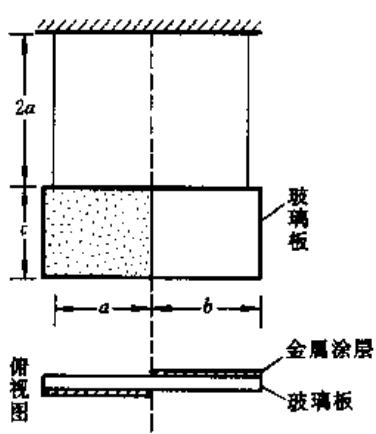
\includegraphics[width=0.2\textwidth]{figures/热图3-2-1.jpg}
\end{center}
\vfill

\newpage
\textbf{3-3} 如热图3-3-1，在真空中有一个质量为 $M$ 的试管，它被质量为 $m$ 的隔板等分为两部分。隔板封闭的那部分有质量为 $n\mathrm{mol}$ , 温度为 $T$ , 摩尔质量为 $\mu$ 的单原子分子理想气体. 放开隔板后, 隔板无摩擦地直立向上移动, 在隔板离开试管顶端后气体方始从试管逸出. 设隔板开始运动时, 试管静止. 试求试管的最终速度.

设重力可忽略。设气体、隔板、试管三者之间的热量交换可忽略。设在隔板离开试管前，气体经历准静态过程。
\begin{center}
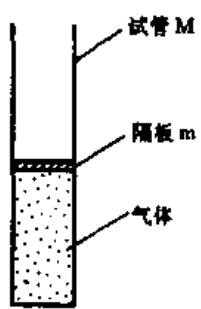
\includegraphics[width=0.15\textwidth]{figures/热图3-3-1.jpg}
\end{center}
\vfill

\textbf{3-4} 在一柱形容器内，有大量相同的小球沿着容器的长度方向往返运动。小球可视为质点，小球之间以及小球与容器端面(与其长度方向垂直)之间作弹性碰撞。小球的速率以及向前还是向后运动都是无规的。可引入"温度"T的概念，它是由小球的平均动能 $\varepsilon$ 定义的，为 $\bar{\varepsilon}=\frac{1}{2}kT$ ，式中k是玻尔兹曼常数。今在容器的一端安装平面弹性活塞，并使活塞缓慢地沿容器长度方向向内推进，运动的小球因与活塞作弹性正碰撞增加了动能，从而使系统的"温度"升高。

上述模型实际上就是单原子分子理想气体一维热运动绝热压缩的微观模型。

试导出在活塞缓慢推进过程中，"温度"T与体积V的关系式(此即单原子分子理想气体的一维绝热过程方程).设重力,引力,各种阻力和摩擦力均可忽略.
\vfill

\newpage
\textbf{3-5} 空腔内的热辐射可以当作光子气来处理．设腔的内表面对光子是完全反射面．

1. 如果在某温度下，腔内热辐射已处于平衡状态，此时光子气的能量密度为 u。试求光子气的压强 p。

2. 试证明 $u$ 只是温度 $T$ 的函数。

3. 试证明 $p \propto T^4$ .

4. 试导出光子气在绝热过程中压强 $p$ 与空腔体积 $V$ 之间满足的关系式(绝热过程方程).
\vfill

\textbf{3-6} 混合理想气体处于温度为 $T$ 的平衡态, 其中任意两个质量分别为 $m_{1}$ 和 $m_{2}$ 的分子之间的相对速度定义为 $\pmb{u} = \pmb{v}_{1} - \pmb{v}_{2}$ , 式中 $\pmb{v}_{1}$ 和 $\pmb{v}_{2}$ 分别是 $m_{1}$ 和 $m_{2}$ 的速度. 试求: 相对速率的方均根值和平均值, 即求 $\sqrt{\overline{u^2}}$ 和 $\overline{u}$ .
\vfill

\newpage
\textbf{3-7} 理想气体处于平衡态，其分子平动动能表为 $E$ ，分子最概然平动动能表为 $E_{\mathrm{p}}$ ，与 $E_{\mathrm{p}}$ 相应的平动速率表为 $v_{0}$ ，试求 $v_{0}$ 与最概然速率 $v_{\mathrm{p}}$ 的比值.
\vfill

\textbf{3-8} 设热气球具有不变的容积 $V_{B} = 1.1 \, \mathrm{m}^{3}$ ，气球蒙皮体积与 $V_{B}$ 相比可忽略不计，蒙皮的质量为 $m_{H} = 0.187 \, \mathrm{kg}$ 。在外界气温 $t_{1} = 20 \, ^{\circ}\mathrm{C}$ ，正常外界大气压 $p_{1} = 1.013 \times 10^{5} \, \mathrm{Pa}$ 的条件下，气球开始升空，此时外界大气的密度为 $\rho_{1} = 1.2 \, \mathrm{kg/m}^{3}$ 。

1. 试问气球内部的热空气的温度 $t_2$ 应为多少, 才能使气球刚好浮起.

2. 先把气球系牢在地面上，并把其内部的空气加热到稳定温度 $t_{3} = 110^{\circ}\mathrm{C}$ ，试问气球释放升空时的初始加速度 a 等于多少？(不考虑空气的阻力。)

3. 将气球下端通气口扎紧，使气球内部的空气密度保持恒定。在内部空气保持稳定温度 $t_{3} = 110^{\circ}\mathrm{C}$ 的情况下，气球升离地面，进入温度恒为 $20^{\circ}\mathrm{C}$ 的等温大气层中。试问，在这些条件下，气球上升到多少高度 h 能处于力学平衡状态。

4. 在上升到第3问中的高度 $h$ 时, 将气球在竖直方向上拉离平衡位置 $10 \mathrm{~m}$ , 然后再予以释放. 试定性叙述气球将作何种运动.
\vfill

\newpage
\textbf{3-9} 取地面为重力势能零点．试估算等温大气的重力势能与热运动能量之比．设大气分子都只有平动和转动的动能已被激发．
\vfill

\textbf{3-10} 把大气看作理想气体，设在大气范围内重力加速度 $g$ 为常量，设海平面 $z = 0$ 处的大气温度为 $T_{0}$

1. 从力平衡观点出发, 试导出 $z$ 处压强随高度的变化率 $\frac{\mathrm{d}p}{\mathrm{d}z}$ 与 $z$ 处的压强 $p$ 和温度 $T$ 的关系.

2. 设大气是等温的，且 $t_{0}=0^{\circ}\mathrm{C}$ ，试计算半数分子处于其下的高度 h.

3. 设大气是绝热的, 且 $t_0 = 0$ ℃, 绝热指数 $\gamma = \frac{7}{5}$ . 试计算大气层的高度 $H$ .
\vfill

\newpage
\textbf{3-11} 设地球的大气等温，温度为 $T$ ，地面附近的分子数密度为 $n_0$ ，大气分子的平均质量为 $m$ .如果认为，在距地面高度为 $\pmb{h}$ 处的大气分子沿某方向（当然不包括会与地面相碰的那些方向）的速度，达到或超过该处人造卫星绕地球作圆运动的速度（在不计空气阻力条件下）时，该分子便能沿此方向逃离大气而去．设地球半径为 $\pmb{R}$ ，地面的重力加速度为 $\pmb{g}$ 试求在 $\pmb{h}$ 处，沿任一允许方向,单位时间通过单位垂直截面逃离大气的分子数.
\vfill

\textbf{3-12} 一根长为 $L$ 的水平粗管与一根竖直细管连接成如热图3-12-1所示的形状。把细管下端插入密度为 $\rho_{f}$ 的液体之中，然后将粗管的管口封住，并使粗管绕细管以恒定的微小角速度 $\omega$ 旋转。已知空气的密度为 $\rho_{u}$ ，细管的体积与粗管相比可以忽略，毛细现象也可忽略。在温度恒定的条件下，试求细管中液面上升的高度 $h$ 。
\begin{center}
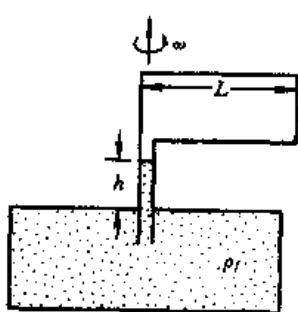
\includegraphics[width=0.2\textwidth]{figures/热图3-12-1.jpg}
\end{center}
\vfill

\newpage
\textbf{3-13} 原子序数为 $Z$ ，原子量为 $A$ 的单质气体，完全电离后形成的等离子体在均匀引力场 $\pmb{g}$ 中处于热平衡状态。设气体密度很小，电离后正、负离子间的局域相互作用可以忽略。

1. 在等温条件下,为了避免宏观的电荷分离(即正离子的数密度与负离子的数密度之比不因位置而变化),试证明必须有均匀电场 $E = -\frac{Am_{p} - m_{e}}{(1 + Z)e}g$ 存在.其中 $m_{p}$ 和 $m_{e}$ 分别是质子和电子的质量.

2. 如果不等温, 但各正、负离子受到的因热运动相互碰撞引起的平均力可认为相同, 试证明也必须有第 1 问的电场 E 存在.

3. 太阳表面附近存在着等离子体, 设其厚度远小于太阳半径, 设太阳表面有均匀分布的电荷 $Q$ , 试在等温、不等温条件下分别求 $Q$ 值.

4. 设太阳表面附近的等离子体是由氢原子电离产生的。试计算 $Q$ 值。已知太阳质量 $M = 2.0 \times 10^{30} \mathrm{~kg}$ 。
\vfill

\textbf{3-14} 从分子某次与其他分子碰撞后开始计算其自由程 $\lambda$ ，它的平均值 $\bar{\lambda}$ 称为平均自由程。设分子间的碰撞具有无后效应性，即在 $\lambda$ 到 $(\lambda + d\lambda)$ 区间与其他分子碰撞的概率与前面已经过的路程 $\lambda$ 无关。试求:

1. 分子经 $\lambda$ 路程尚未被碰撞的概率 $F(\lambda)$ ，以及分子自由程为 $\lambda$ 的概率密度（也称为自由程的分布函数） $f(\lambda)$ .

2. 分子在某次碰撞后, 先经无碰撞的路程 $\lambda_0$ , 再经 $\lambda$ 路程未被碰撞的概率 $F^*(\lambda_0, \lambda)$ , 以及不计 $\lambda_0$ 的平均自由程 $\bar{\lambda}(\lambda_0)$ .
\vfill

\newpage
\textbf{3-15} 理想气体处于平衡态, 分子热运动平均速率为 $\bar{v}$ , 平均自由程为 $\bar{\lambda}$ , 把 $t = 0$ 时刻某分子所在位置取为坐标原点 O. 试问经过多长时间 t, 该分子所在位置与原点 O 相距为 R.设理想气体占据的容器空间足够大, 设 $R \gg \bar{\lambda}$ , 设该分子在本题讨论的时间范围内未与容器壁相碰.最后, 已知 $\bar{v} = 5.0 \times 10^{2} \, \mathrm{m/s}, \bar{\lambda} = 3.0 \times 10^{-7} \, \mathrm{m}, R = 2 \, \mathrm{m}$ , 试给出 t 的具体数值.
\vfill

\textbf{3-16} 某混合理想气体包含A和B两种分子，已知A和B分子的质量、有效直径和数密度分别为 $m_{\mathrm{A}}$ 和 $m_{\mathrm{B}}, d_{\mathrm{A}}$ 和 $d_{\mathrm{B}}$ 以及 $n_{\mathrm{A}}$ 和 $n_{\mathrm{B}}$ 。试求在温度为 $T$ 的平衡态，两种分子各自的平均自由程 $\bar{\lambda}_{\mathrm{A}}$ 和 $\bar{\lambda}_{\mathrm{B}}$ 。
\vfill

\newpage
\textbf{3-17} 在阴极射线管中，即使管腔被抽成很高的真空度，也总是还有一些残余的空气存在。因此，从阴极射出的高速电子在通过管腔时，总有一部分因与空气分子相碰而不能直接射到荧光屏上。设阴极射线管工作时，管腔内的温度为 $27^{\circ}\mathrm{C}$ ，管腔的长度为 $20\mathrm{cm}$ 。为了保证有 $90\%$ 的电子能够不经碰撞直接射到屏上，试问管腔需抽到多高的真空度（用管腔内空气的压强表示）。已知空气分子的有效直径为 $3.0 \times 10^{-10}\mathrm{m}$ 。
\vfill

\textbf{3-18} 设气体分子的热运动速度分布在速度空间具有球对称性，速率分布函数为 $f(v)$ ，分子数密度为 $n$ 。试证明:

1.速率在 v 到 $\left(v + dv\right)$ 的分子, 单位时间与单位面积容器壁碰撞的分子数为 $\frac{1}{4}\left(nf(v)\mathrm{d}v\right)v$.

2. 全部气体在单位时间内与单位面积容器壁碰撞的分子数为 $\frac{1}{4} n\bar{v}$ , 其中 $\bar{v}$ 的分子的平均速率.
\begin{center}
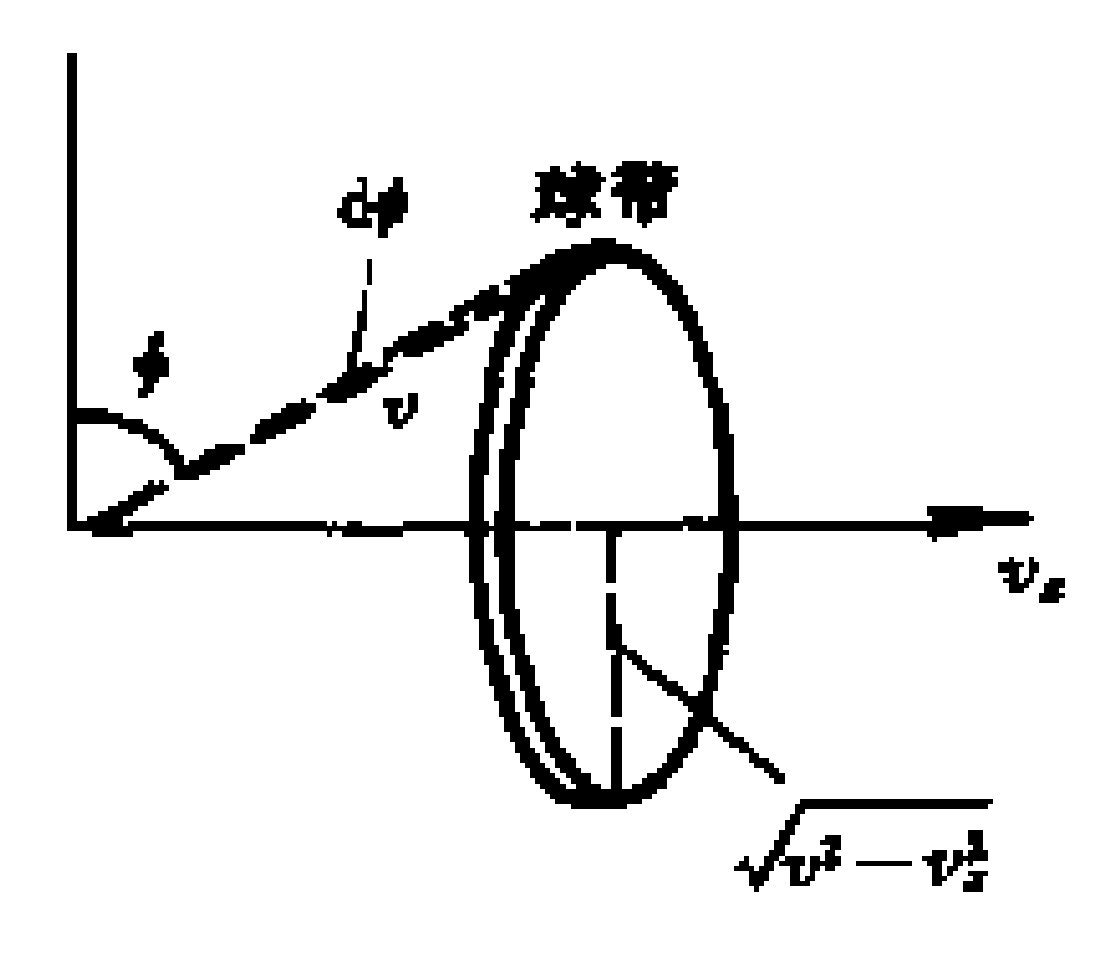
\includegraphics[width=0.3\textwidth]{figures/热图3-18-1.jpg}
\end{center}
\vfill

\newpage
\textbf{3-19} 如热图3-19-1,在温度为 $1000^{\circ}\mathrm{C}$ 的真空加热室中蒸发产生的铍原子(原子量为 9)气体经小孔逸出,透过准直狭缝形成原子束后,进入长度为 1 m 的真空大容器中,容器的右壁与原子束垂直.

1. 试求原子束中原子的速率分布, 平均速率和方均根速率.

2. 原子束中的原子进入真空容器后，将与残存的稀薄空气分子发生碰撞。设原子束行进1 m 后, 其强度(单位时间内通过的原子数) 减小为原来的 $\frac{1}{e}$ . 已知真空容器的温度为 300 K, 铍原子与空气分子的碰撞截面为 $10^{-20} ~\mathrm{m}^{2}$ , 忽略铍原子之间的碰撞. 试问真空容器中残存空气的压强是多少?

3. 铍原子每行进 1 m 所需的平均时间 $\bar{\tau}$ 是多少?

4. 设铍原子束刚进入真空容器时的粒子数密度为 $n_0 = 10^{10} \mathrm{~cm}^{-3}$ , 设铍原子与容器壁作完全非弹性碰撞. 试估计因铍原子束与容器壁碰撞对后者所施加的压强.
\begin{center}
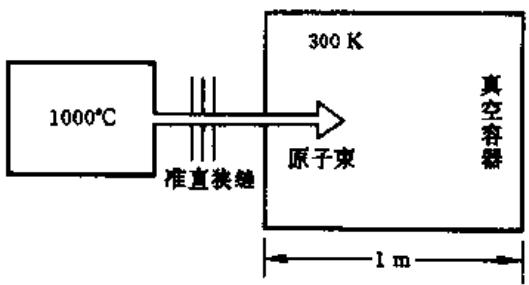
\includegraphics[width=0.3\textwidth]{figures/热图3-19-1.jpg}
\end{center}
\vfill
\newpage

\textbf{3-20} 在气象学中，降雨量是指雨区地面雨水的累加高度。今在离地面足够高处有一片厚度可忽略不计的降雨云层，单位时间的降雨量 $Q$ 为常量。假设雨滴在垂直下落过程中近似保持球体形状，半径均为 $R$ ，空气对雨滴的阻力的大小与雨滴的速度大小成正比，比例系数为常量 $\alpha$ 。

1. 若在雨区有一飞虫以速率 u 作水平飞行, 飞虫也近似看作球体, 半径为 r, 试在降雨稳定的持续时间内, 确定飞虫在雨中的平均自由程(即飞虫每相邻两次与雨滴碰撞之间飞过的路程之平均值) 的上限.再用 $Q = 10 \, \mathrm{cm/h}, R = 1.00 \, \mathrm{mm}, \alpha = 3.00 \times 10^{-3} \, \mathrm{g/s}, u = 10.0 \, \mathrm{m/s}, r = 4.00 \, \mathrm{mm}$ 等数据计算此上限。

2. 设在某段高度范围内雨滴降落速度可以认为是常量 $v$ ，而飞虫在该区域恰以速率 $u = v$ 飞行。如果飞虫朝任一空间方向飞行的可能性都相同，试问在不同的飞行方向上，飞虫在雨中的平均自由程是否相同？如果相同，试算出这相同的平均自由程；如果不相同，试计算这些平均自由程的平均值。

\vfill

\newpage
\textbf{3-21} 气体粘滞系数的测定.

把待测气体充入容积为 $V_{0}$ 的烧瓶中，使其压强 $p_{b}$ 大于外界大气压强 $p_{0}$ ，其温度则与外界温度 $T_{0}$ 一致。烧瓶口外连接长为 $L$ 、半径为 $r$ 的水平细圆管与大气相通。细管与烧瓶连接处有阀门，先关闭。打开阀门后瓶内气体经细管向外流出，经过 $\Delta t$ 时间后再将阀门关闭，测出瓶内气体压强为 $p_{e}$ ，由此便可确定该气体的粘滞系数 $\eta$ 。设整个过程中，烧瓶、细管、外界处处温度相同且保持不变。试导出 $\eta$ 的计算公式。

某次实验以二氧化碳为待测气体, 有关实验数据为, $V_{0} = 1.0 \mathrm{~L}, p_{b} = \frac{1600}{760} \mathrm{atm}, P_{0} = \frac{735}{760} \mathrm{atm}, t_{0} = 15^{\circ} \mathrm{C}, L = 10 \mathrm{~cm}, r = 0.050 \mathrm{~mm}, \Delta t = 22 \mathrm{~min}, p_{e} = \frac{1350}{760} \mathrm{atm}$ , 试利用导出的公式计算二氧化碳的粘滞系数 $\eta$ .

\vfill

\textbf{3-22} 试证明两杯成分相同而体积和温度不同的液体混合后总体积不变，设该液体的体积随温度($^{\circ}\mathrm{C}$)线性地变化，且在混合过程中与外界绝热。
\vfill

\newpage
\textbf{3-23} 冬季湖面上的冰经两天的时间，厚度从 $20\mathrm{mm}$ 增为 $40\mathrm{mm}$ ，在此期间冰层底部与顶部的平均温差为 $8.0\mathrm{K}$ 。设冰的密度为 $920\mathrm{kg} / \mathrm{m}^3$ ，冰的熔解热为 $3.20\times 10^{5}\mathrm{J / kg}$ 。试估算冰的热传导率 $k$ 。
\vfill

\textbf{3-24} 用同一种物质铸造出质量相同的实心球A和立方体B，将它们加热到 $220^{\circ}\mathrm{C}$ ，然后都在 $20^{\circ}\mathrm{C}$ 的环境中冷却。设A和B的热损耗率(单位时间向外散发的热量)均与表面积以及各自与环境的温度差成正比，且比例系数相同。试用A在降温过程中的温度 $\tau_{\mathrm{A}}$ 来表述B在降温过程中的温度 $\tau_{\mathrm{B}}$ 。
\vfill

\newpage
\textbf{3-25} 半径为 $R_{1}$ 的球体内有供能装置，使之成为高温热源。在球体之外包着导热的匀质球壳层A，它的内半径为 $R_{1}$ ，外半径为 $R_{2}$ ，导热系数处处相同，为常量 $k$ 。球壳层外是另一均匀热介质。当达到稳定的热传导时，内球温度恒为 $T_{1}$ ，球壳层 $A$ 外的温度恒为 $T_{2}$ ，且 $T_{2} < T_{1}$ 。

1. 试确定球壳层 A 中温度的径向分布。

2. 试求单位时间内, 内球中的供能装置应提供的能量.
\vfill

\textbf{3-26} 如热图3-26-1，长为 $2l$ ，半径为 $\pmb{r}$ 的圆柱形保险丝与电路中的两个电阻块A和B连接．设A和B与周围环境具有相同的恒定温度 $T_{c}$ .设保险丝中通过稳恒电流 $I$ ，保险丝已达到热稳定状态.设保险丝中任一正截面上的温度都相同，记为 $(T_{c} + T)$ ，不同正截面上的温度不同，若某正截面与 A 相距为 x，它的温度表为 $T(x)$ 。设保险丝的电阻率为 $\rho$ ，设保险丝沿其长度方向（即 x 方向）的热传导率为 $\lambda$ ，设保险丝单位时间通过其侧面单位面积向外界散发的热量为 CT，其中 C 为常量。

试求保险丝上的温度分布，即求 $T(x)$ 函数。试就 $l \gg \left(\frac{\lambda r}{2C}\right)^{\frac{1}{2}}$ 的所谓长保险丝情形，计算能使长保险丝熔断的电流强度，设保险丝材料的熔点为 $T_{m}$。
\begin{center}
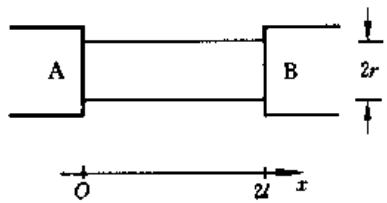
\includegraphics[width=0.3\textwidth]{figures/热图3-26-1.jpg}
\end{center}
\vfill


\newpage
\textbf{3-27} 沿 $x$ 轴在 $x = 0$ 到 $x = L$ 之间放一段长为 $L$ 截面积为 $S$ 的均匀柱体，它与外界绝热。 $t = 0$ 时， $x = 0$ 处的温度为 $T_{1}, x = L$ 处的温度为 $T_{2}$ ，且 $T_{1} > T_{2}$ ，其间温度 $T$ 线性地分布。设柱体的热传导率 $k$ ，比热 $c$ 及密度 $\rho$ 均为常量，各处的热膨胀均可略。试导出 $t$ 时刻 $x$ 处温度 $T(x, t)$ 的积分表达式。
\vfill

\textbf{3-28} 在温度为 $T$ 的恒温热源中有一导热容器，它被隔板分成体积均为 $V$ 的左、右两部分，隔板上有一小孔，面积为 $A$ ，开始时 $(t = 0)$ ，左方装有摩尔质量为 $\mu_{1}$ 的 $\nu \mathrm{mol}$ 理想气体，右方装有另一种摩尔质量为 $\mu_{2}(\mu_{2} \neq \mu_{1})$ 的 $\nu \mathrm{mol}$ 理想气体。由于孔很小，虽然板两侧不断有分子交换，但仍可假定在任一时刻系统都处于平衡态。

1. 试求隔板左、右两侧气体的密度 $\rho_{L}, \rho_{R}$ 各自随时间 $t$ 的变化关系。

2. 试计算最后达到 $\rho_{L} = \rho_{R}$ 时，气体系统的熵的增量。
\vfill

\newpage
\textbf{3-29} 利用布朗运动的实验可以粗略测量阿伏伽德罗常数 $N_{A}$

作布朗运动的微粒系统可以看作是在计及浮力的重力场中达到平衡态的巨分子系统,其数密度遵循玻尔兹曼分布律．设在某实验中，半径 $r=2.12\times10^{-7}$ m，质量密度 $\rho=1.194\times10^{3}$ kg/m$^{3}$ 的球形布朗粒子，悬浮在密度 $\rho_{0}=1.0\times10^{3}$ kg/m$^{3}$ 、温度 T=273 K 的液体中．在高度相距为 $\Delta h=3.0\times10^{-5}$ m 的两处，测得布朗粒子的数密度之比为 $n_{1}:n_{2}=2.08$ .

试求 $N_{A}$ 。
\vfill
\newpage

\textbf{3-30} 流体中悬浮小颗粒的布朗运动尽管很复杂，但它在不断被碰撞中像一个大分子一样按能量均分定理获得了自己的运动能量，这就为讨论它的位移方均量提供了基础。

为讨论方便, 考虑在 $x$ 方向的一维布朗运动. 小颗粒在 $x$ 方向的碰撞净作用力 $F(t)$ 和阻尼力 $f(t)$ 的作用下运动. 若 $t = 0$ 时刻小颗粒处于 $x = 0$ 位置, 那么可以肯定, 在尔后任何时刻 $t$ 都有 $\overline{x(t)} = 0$ , 但 $\overline{x^2(t)}$ 必不为零. 由于热平衡是动态平衡, $F(t)$ 将在零值左右波动, 但必有 $\overline{F(t)} = 0$ . 设小颗粒是半径为 $R$ 的球体, 它所受流体的粘滞阻力为 $f(t) = -6\pi R\eta v_x$ , 其中 $v_x$ 是小颗粒在 $x$ 方向的运动速度, $\eta$ 是流体的粘滞系数. 设实验中所采用的布朗运动小颗粒的质量 $m \ll 6\pi R\eta$ .

1. 试用牛顿第二定律,证明在温度为 T 时有很好的近似解

$$
\overline{x^2(t)} = \frac{kT}{3\pi R\eta}t
$$

式中 $k$ 为玻尔兹曼常量.

2. 取 $R = 5.0 \times 10^{-6} \mathrm{~m}$ 的细小油珠, 测量它悬浮在氮气中时沿水平方向 $x$ 的布朗运动. 每隔 $5 \mathrm{~s}$ 测量一次油珠的 $x$ 坐标, 每两个相邻的 $x$ 值之差记为 $\Delta x$ . 实验中测出 695 个 $\Delta x$ 值, 按 $\Delta x$ 的大小分为 27 组, 每一组中的 $\Delta x$ 相同, 每一组中 $\Delta x$ 的个数记为 $n$ , 详如下表.
\begin{center}
    \begin{tabular}{|c|c|c|c|c|c|c|c|c|}
    \hline
    $\Delta x/(10^{-6} \mathrm{m})$ & $-13$ & $-12$ & $-11$ & $-10$ & $-9$ & $-8$ & $-7$ & $-6$ \\
    \hline
    $n$ & $0$ & $2$ & $4$ & $5$ & $10$ & $14$ & $22$ & $26$ \\
    \hline
    $\Delta x/(10^{-6} \mathrm{m})$ & $-5$ & $-4$ & $-3$ & $-2$ & $-1$ & $0$ & $1$ & $2$ \\
    \hline
    $n$ & $29$ & $35$ & $45$ & $49$ & $63$ & $75$ & $60$ & $54$ \\
    \hline
    $\Delta x/(10^{-6} \mathrm{m})$ & $3$ & $4$ & $5$ & $6$ & $7$ & $8$ & $9$ & $10$ \\
    \hline
    $n$ & $45$ & $37$ & $31$ & $27$ & $20$ & $16$ & $9$ & $8$ \\
    \hline
    $\Delta x/(10^{-6} \mathrm{m})$ & $11$ & $12$ & $13$ & & & & & \\
    \hline
    $n$ & $6$ & $3$ & $0$ & & & & & \\
    \hline
    \end{tabular}
\end{center}
实验是在 $15^{\circ}$ C 下进行的，此时氮气的粘滞系数 $\eta=1.73\times10^{-5}$ Pa·s.

试计算玻尔兹曼常量 k 的值。
\vfill


